\documentclass[10 pt,usenames,dvipsnames, oneside]{article}
\usepackage{../../../modelo-fracoes}
\graphicspath{{../../../Figuras/licao01/}}



\begin{document}

\begin{center}
  \begin{minipage}[l]{3cm}

\includegraphics[width=2cm]{logo}    
\end{minipage}\hfill
\begin{minipage}[r]{.8\textwidth}
 {\Large \scshape Atividade: As estrelinhas de Alice}  
\end{minipage}
\end{center}
\vspace{.2cm}

\ifdefined\prof
\begin{goals}
\begin{enumerate}
    \item       Reconhecer a equipartição em um modelo linear.
    \item       Reconhecer a quarta parte como a metade da metade.
\end{enumerate}
\tcblower
\begin{itemize} %s
   \item No final deste volume estão disponíveis materiais para reprodução. Esta atividade necessita deste material.
   \item Recomenda-se que esta atividade seja desenvolvida em grupos de quatro alunos.
   \item       Cada grupo deve receber um pedaço de barbante de, aproximadamente, 1m e quatro enfeites (todos iguais).
    \item       Os quatro enfeites precisam ser confeccionados antes da realização da tarefa. Sugerem-se estrelas, cujos modelos estão disponíveis para reprodução no final do livro. No entanto, segundo a avaliação do professor, os enfeites podem ser outros, desde que sejam os 4 congruentes.
    \item       Como sugestão, se possível, solicitar aos alunos que confeccionem os enfeites, por exemplo, associando esta atividade com geometria, com a abordagem de grandezas e medidas, com a disciplina de artes ou envolvendo culturas artesanais populares.
    \item       A equipartição do barbante não deve ser obtida a partir da medida do barbante, mas por sucessivas dobras do barbante sobre ele mesmo, como ilustrado na resposta da atividade. Tal discussão também  será útil na abordagem de frações equivalentes na Lição 4.
    \item       A manipulação e a dobra do barbante devem sustentar a discussão para a identificação da       ``metade da metade'' com a       ``quarta parte'' do barbante. Nesse caso, a identificação se dará pela sobreposição das partes.
      \item Nossa experiência aplicando esta atividade tem mostrado um efeito emocional positivo em permitir que os estudantes realmente confeccionem os enfeites.
\end{itemize} %s

\end{goals}

\bigskip
\begin{center}
{\large \scshape Atividade}
\end{center}
\fi

Alice quer enfeitar a sala de aula e pretende pendurar os enfeites utilizando pedaços de barbante. Para que os enfeites fiquem todos na mesma altura, quer cortar o barbante em pedaços iguais. Ajude Alice a cortar o barbante (você receberá o barbante do seu professor).

\begin{center}
    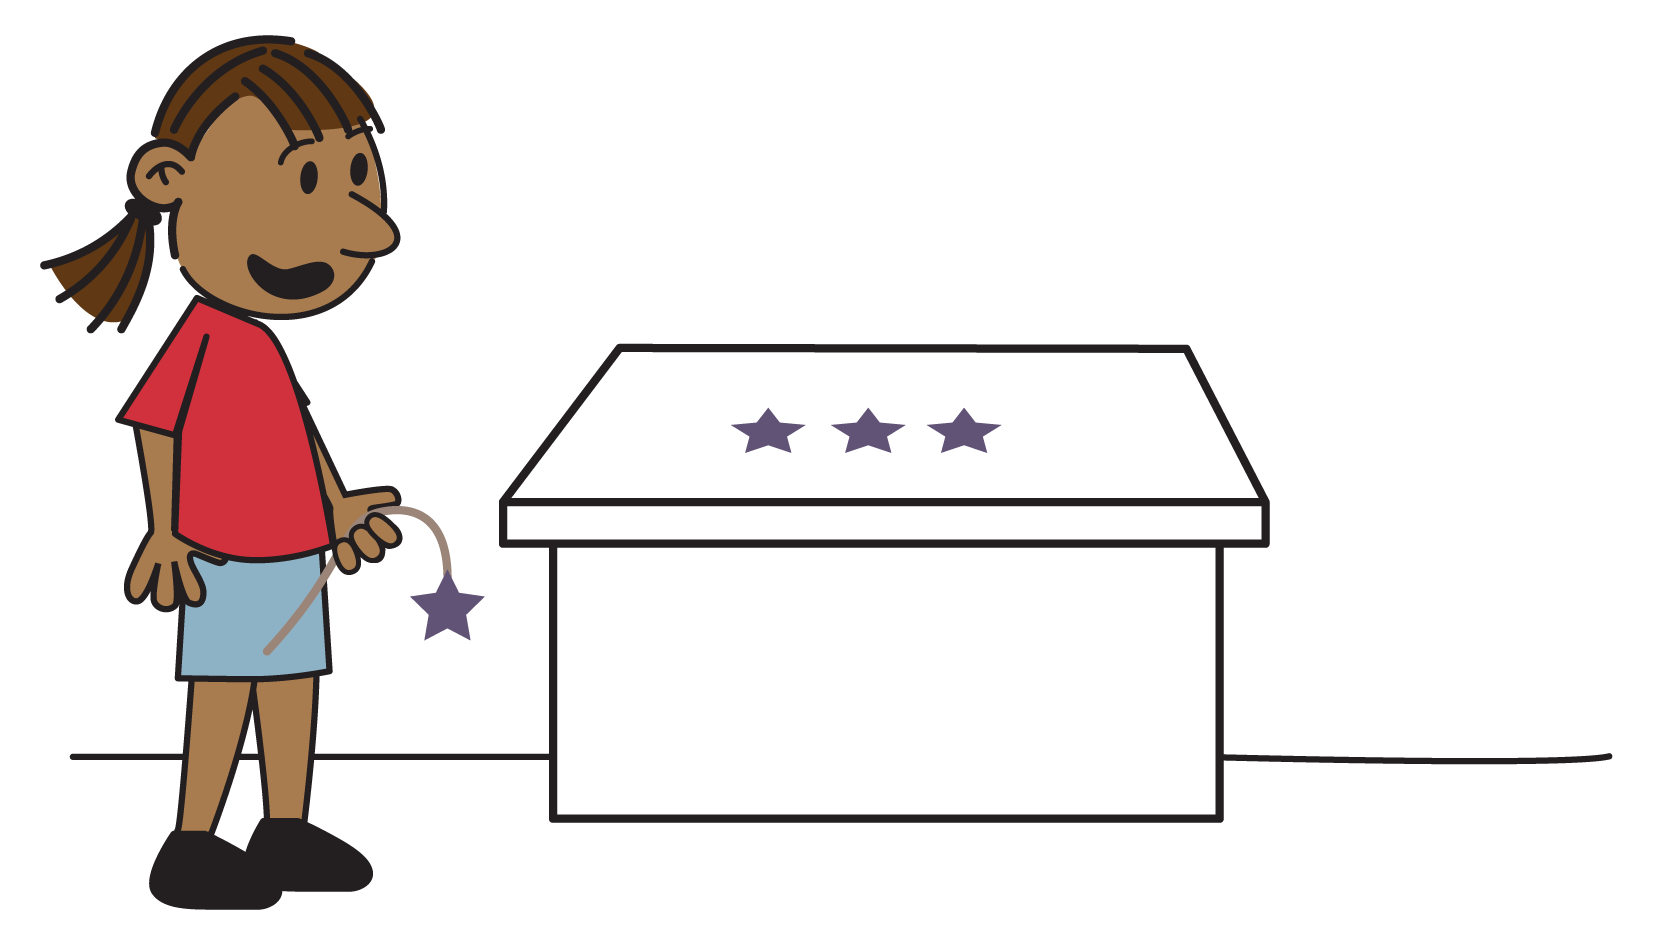
\includegraphics[width=350pt, keepaspectratio]{ativ3_fig01.png}
  \end{center}

\ifdefined\prof

\begin{solucao}

Uma maneira de se cortar o barbante é dobrar ao meio e depois dobrar novamente ao meio, obtendo quatro partes iguais, como ilustrado na figura a seguir.
  \begin{center}
  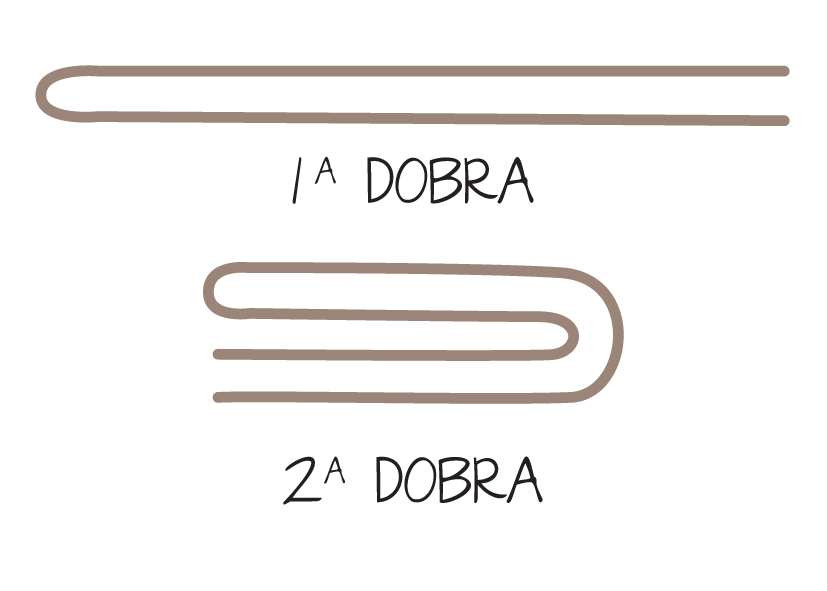
\includegraphics[width=200pt, keepaspectratio]{ativ3_fig03.png}
  \end{center}

\end{solucao}
\fi

\end{document}